% Front cover: full-bleed image (assets/front-cover.png) with the title in the
% clear top band and the author in the lower band. Injected before the body via
% pandoc --include-before-body. Text colour is the dark slate (gbNode) so it
% reads on the light background of the artwork.
\graphicspath{{assets/}{../assets/}{./}}
\begin{titlepage}
\thispagestyle{empty}
\begin{tikzpicture}[remember picture, overlay]
  % full-bleed artwork
  \node[anchor=center, inner sep=0pt] at (current page.center)
    {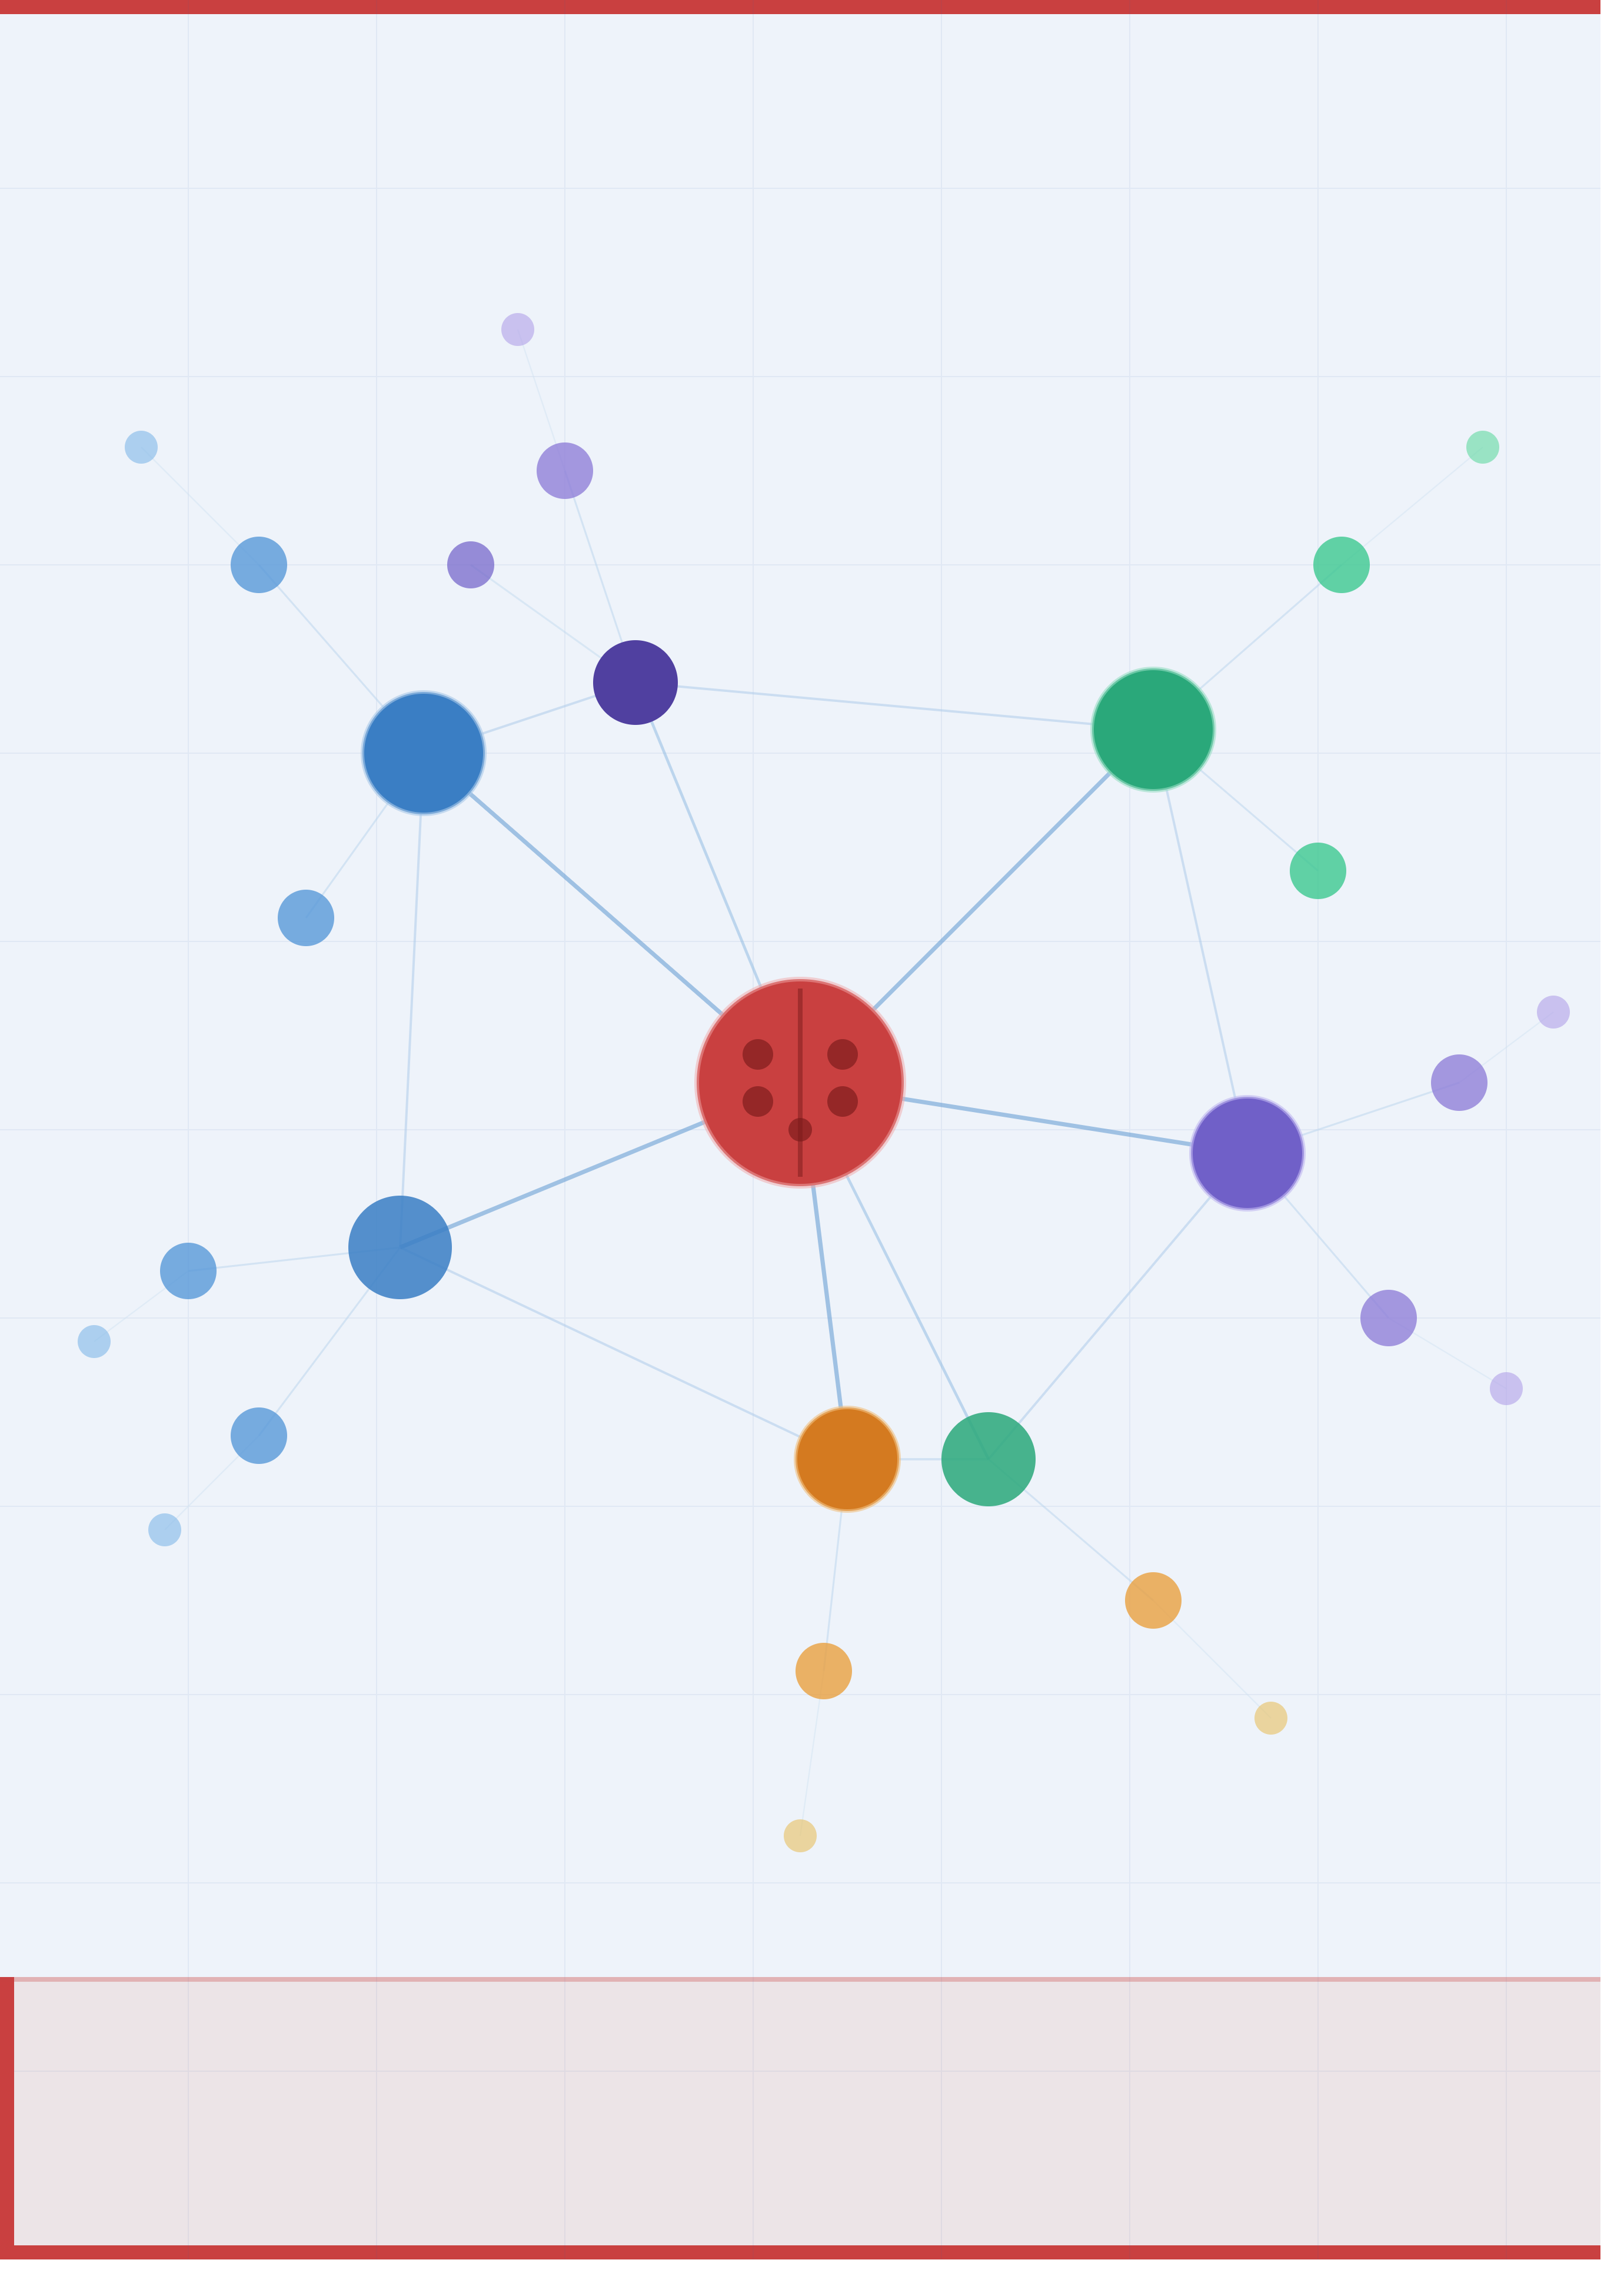
\includegraphics[width=\paperwidth, height=\paperheight]{front-cover.png}};
  % title + subtitle in the clear top band
  \node[anchor=north, text width=0.84\paperwidth, align=center]
    at ([yshift=-1.7cm]current page.north) {%
      {\sffamily\bfseries\color{gbNode}\fontsize{30}{35}\selectfont
        Graph for the Data You Already Own\par}%
      \vspace{10pt}%
      {\sffamily\color{gbNode!85}\fontsize{14}{18}\selectfont
        A short book on Graph Data for Working\\
        Data Engineers, with LadybugDB\par}%
  };
  % author in the lower band
  \node[anchor=south]
    at ([yshift=1.3cm]current page.south)
    {\sffamily\color{gbNode}\Large Jaganadh Gopinadhan (Jagan)};
\end{tikzpicture}
\end{titlepage}

% Copyright / license page (verso of the cover, before the table of contents).
\thispagestyle{empty}
\vspace*{1.4cm}
{\small\sffamily\setlength{\parindent}{0pt}\setlength{\parskip}{1.2ex}

\textbf{Graph for the Data You Already Own}\\
A short book on Graph Data for Working Data Engineers, with LadybugDB

Copyright \textcopyright\ 2026 Jaganadh Gopinadhan.\\
Contact: \href{mailto:jgopinadhan@acm.org}{jgopinadhan@acm.org}

\textbf{Text and figures.} This work is licensed under a Creative Commons
Attribution-ShareAlike 4.0 International License (CC BY-SA 4.0). You are free
to share and adapt the material for any purpose, including commercially,
provided you give appropriate credit and license your derivative works under
the same terms. Full license: \url{https://creativecommons.org/licenses/by-sa/4.0/}

\textbf{Code.} All source code in this book (the Cypher queries, the shell
scripts, and the Python in Appendix D) is provided under the MIT License:

{\footnotesize
MIT License

Copyright \textcopyright\ 2026 Jaganadh Gopinadhan

Permission is hereby granted, free of charge, to any person obtaining a copy of
this software and associated documentation files (the ``Software''), to deal in
the Software without restriction, including without limitation the rights to
use, copy, modify, merge, publish, distribute, sublicense, and/or sell copies of
the Software, and to permit persons to whom the Software is furnished to do so,
subject to the following conditions:

The above copyright notice and this permission notice shall be included in all
copies or substantial portions of the Software.

THE SOFTWARE IS PROVIDED ``AS IS'', WITHOUT WARRANTY OF ANY KIND, EXPRESS OR
IMPLIED, INCLUDING BUT NOT LIMITED TO THE WARRANTIES OF MERCHANTABILITY, FITNESS
FOR A PARTICULAR PURPOSE AND NONINFRINGEMENT. IN NO EVENT SHALL THE AUTHORS OR
COPYRIGHT HOLDERS BE LIABLE FOR ANY CLAIM, DAMAGES OR OTHER LIABILITY, WHETHER IN
AN ACTION OF CONTRACT, TORT OR OTHERWISE, ARISING FROM, OUT OF OR IN CONNECTION
WITH THE SOFTWARE OR THE USE OR OTHER DEALINGS IN THE SOFTWARE.\par}

LadybugDB, Kùzu, Neo4j, and other product names are trademarks of their
respective owners.
\par}
\clearpage
